\documentclass{article}
\usepackage[vmargin=18mm]{geometry}
\usepackage{listings}
\usepackage[utf8]{inputenc}
\usepackage{graphicx}
\usepackage{booktabs}
\usepackage{mapping-tutorial}
\usepackage[lastexercise]{exercise}
\usepackage[ddmmyyyy]{datetime}


\renewcommand{\ExerciseListName}{Exercise}
\setlength{\ExerciseSkipBefore}{1\baselineskip}
\setlength{\ExerciseSkipAfter}{1\baselineskip}

\renewcommand{\dateseparator}{-}

\newcommand{\gabmap}{\href{http://www.gabmap.nl/}{Gabmap}}

\title{Making maps for \gabmap{}}
%\author{Çağrı Çöltekin}
%\date{\small{\today,~\currenttime}}
\date{}

\lstset{basicstyle=\tt\color{blue}}


\begin{document}
\maketitle{}

\gabmap{} uses information provided in a KML file to visualize the
dialect data on maps.  The
\href{http://en.wikipedia.org/wiki/Keyhole_Markup_Language}{KML} is a
popular format for storing geographical information. Many cartography
applications, including popular \href{https://maps.google.com/}{Google
maps}, and \href{http://http://www.google.com/earth/}{Google earth},
can import and export data in KML format.

In this tutorial we will create a simple map in KML format to be used
with \gabmap{}.

Before we start creating our map, a note on how \gabmap{} uses
information provided in KML files is in order. KML files can contain
detailed information about the mapped area and its visualization.
However, \gabmap{} uses only \emph{points} and \emph{polygons} within
these objects. Typically, you will have a number of points marking the
data-collection locations, and a single polygon marking the borders of
the area you are interested in. \textbf{It is important to name the
locations in your map exactly as you name them in your data files}.

Most commonly used application for preparing maps for \gabmap{} is
\href{http://http://www.google.com/earth/}{Google Earth} or online
\href{https://maps.google.com/}{Google maps}.  We will only cover how
to make maps using the Google maps here. If you'd like to use Google
Earth, you may find the RuG/L04 tutorial at
\url{http://www.let.rug.nl/kleiweg/L04/kml/manual.html} useful.  You
can also use any other application that produces a KML document. In
case you have a map saved in a different format we point you to two
converters that can convert from many different file formats to KML.
The free application \href{http://www.gpsbabel.org/}{GPSBabel}
converts to and from many different geographic data formats, and
includes flexible ways to filter the data.  The second one is the
online converter available at \url{http://geoconverter.hsr.ch/}. 

For the rest of this tutorial we will focus on creating a map of
Belgium to be used in Gabmap. To use this option you need a modern
browser, and a Google account.

First, you need to point your browser to
\url{https://maps.google.com/} and log in. First, you should pan into
an area that covers Belgium. You should have a view similar to this:

\begin{center}
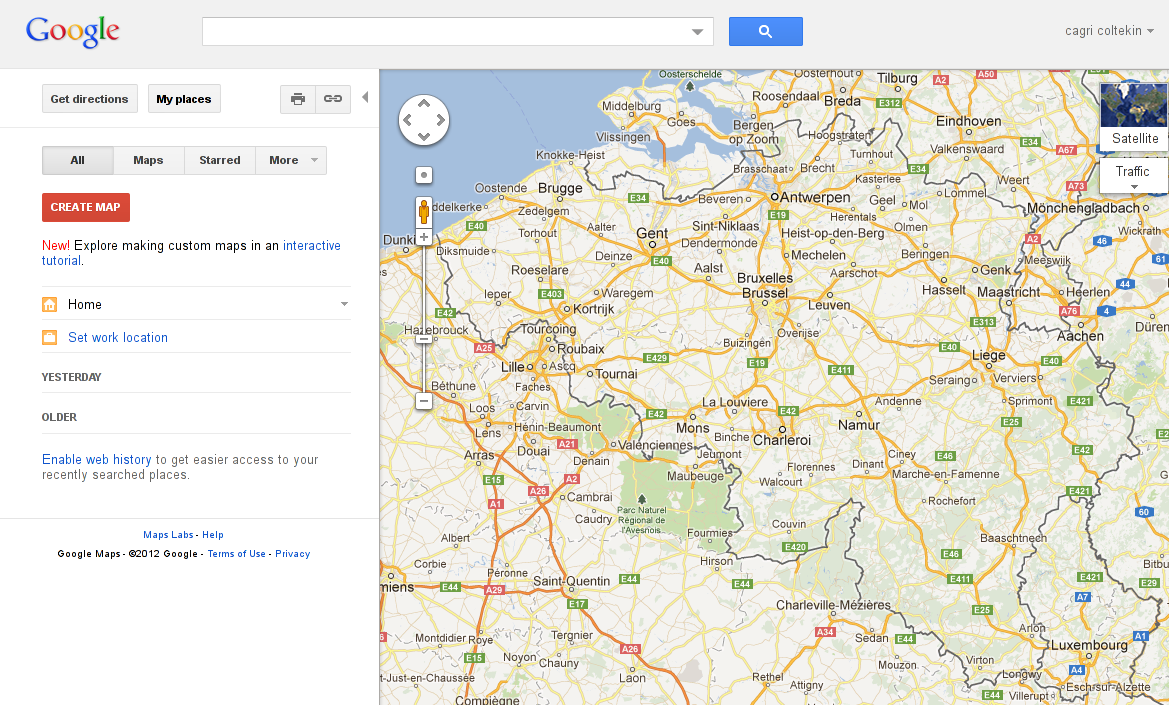
\includegraphics[width=\textwidth]{images/google-maps-start.png}
\end{center}

Now, click to \textsc{create map} button. You will be asked for a
title and an optional description. You can also choose whether you'd
like to keep your map private or share it. Give a name to your map,
such as `Belgium'. Click \textsc{Save} button above the title to save
your map. It is a good idea to save your map time to time while
working on it.

You should also be seeing a set of buttons on the upper-left corner of
the map.

\begin{center}
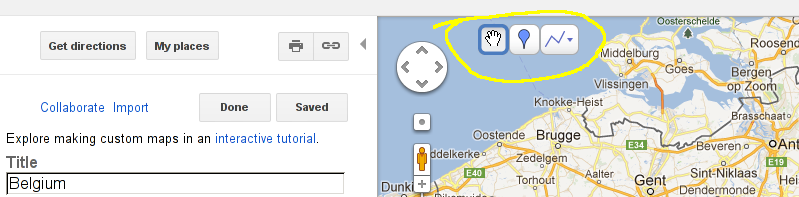
\includegraphics[width=\textwidth]{images/google-maps-tools.png}
\end{center}

We will be using the second one from the left for marking locations,
`\emph{placmarks}', and the third one for adding borders.

You can add place marks in two ways. First, you can select the place
mark tool, and click on the location you want to mark. A new dialog
will appear so that you can give a name to your place mark. 

Second, you can search the place you like to record using the search
box above the map. Once you found the city or spot you are interested
in, click the link `\emph{Save to map}'. You will be presented with a
select box where you can select among the maps you are created, and
click to \textsc{Save} to include the place mark in the selected map.

\begin{Exercise}
Using `placemark' tool mark Brussels on the map, on the map you've
just created.
\end{Exercise}

\begin{Exercise}
Search for Leuven on Google maps, and add the place mark that shows the
center of Leuven to your map.
\end{Exercise}

Your map after adding these two place marks should look like the
following image:

\begin{center}
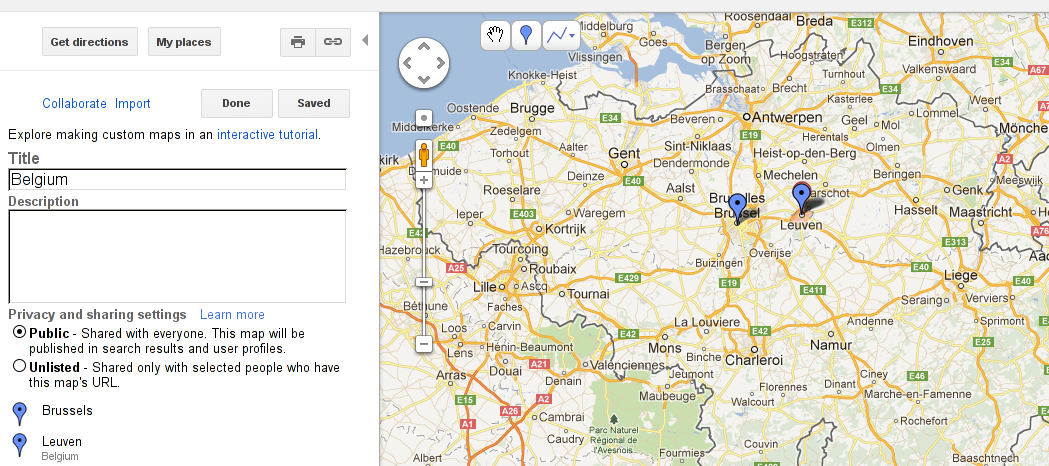
\includegraphics[width=\textwidth]{images/google-maps-placemarks.png}
\end{center}

You can drag your place marks on the map if you want to move them. You
can also edit the associated information about your place marks, but
only the name and the coordinates of a place mark will be used by
\gabmap{}.

\begin{Exercise}
Add five major cities of your choice in Belgium to your map.
\end{Exercise}

The next step is to create a polygon that marks the borders of the
area we are interested in. For this we click on the right-most button
on the upper-left corner of the map, and from the drop-down box, we
choose \textsc{Draw a shape} option. Now, you should be seeing a closed
shape on the button. Now clicking on the map will allow you to mark
corners of a polygon. Once you are done with the last
point, double clicking to the map will close the polygon, and you will
be asked for a name, and an optional description. Note that, \gabmap{}
does not use the name or the description of a polygon.

The following image shows the result of a somewhat crude tracing of
Belgian borders. 

\begin{center}
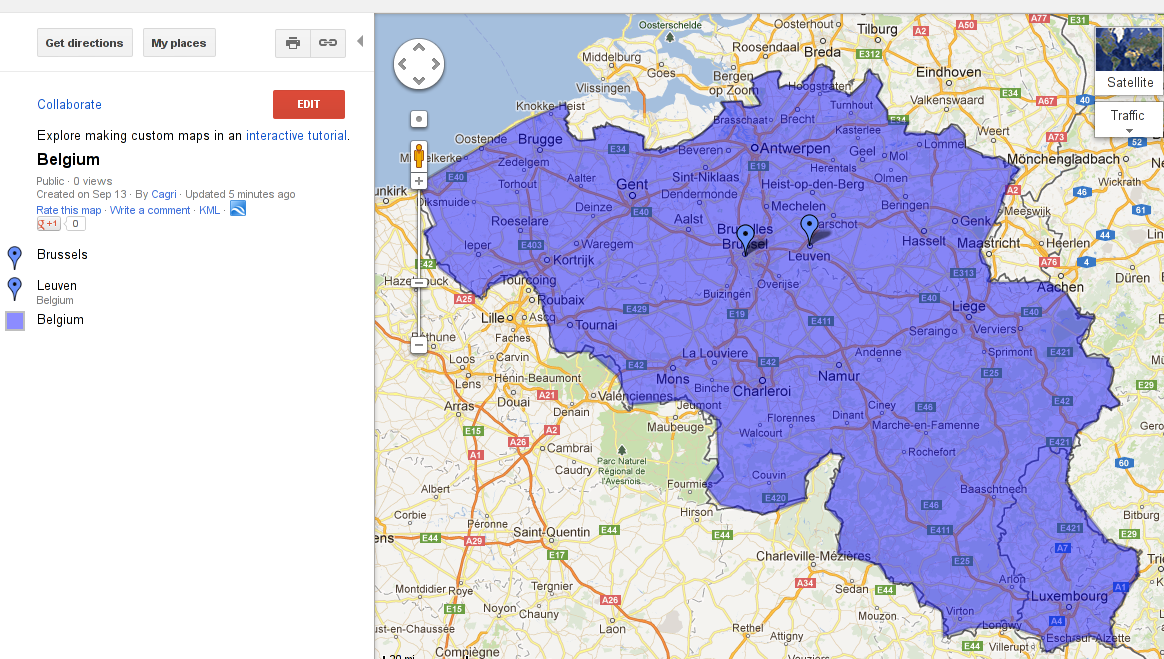
\includegraphics[width=\textwidth]{images/google-maps-borders.png}
\end{center}

\begin{Exercise}
Replicate the above image (an even more coarse trace should be more than
fine for this exercise).
\end{Exercise}

We are ready to save our map as a KML file. First, do not forget
to save your map, and click to \textsc{Done}. Here is what you
should see on the left panel of Google maps:

\begin{center}
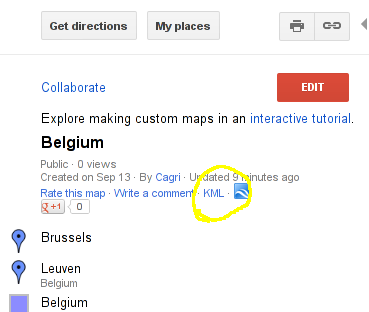
\includegraphics[width=0.5\textwidth]{images/google-maps-kml.png}
\end{center}

Now click on \emph{KML}, and instruct your browser to save it. You
have just created a map that you can use with \gabmap{}.

One last tip: if you already have a KML file, you can first upload it
while creating the map, and edit it as needed.
\end{document}
